\chapter{Operative System Interface}
Once the fundamental process of programming the FPGA is understood, the next step is to explore how to fully exploit the capabilities of the SoM. This chapter provides a foundational overview, but it represents only a fraction of what can be achieved.

Within this chapter it is proposed the same blinking project, but the programming of the FPGA is performed directly by the uP. This latter steps need the configuration of a custom OS through Petalinux SDK. The system is said to be custom because at the end of the procedure, the OS will have enabled only the needed packages, thus it will results in a more lighter implementation with respect to an already available OS. To program the FPGA directly from the OS, a configuration file in a binary format is needed, thus the .bit file has to be converted. There are few ways to do so, but certainly the easiest is to add to the Vivado output the creation of the .bin file. From the previous project, go to \textbf{Settings} → \textbf{Bitstream} → \textbf{bin\_file} → \textbf{Apply} and regenerate the bistream. The .bin file should be saved in the same folder as the .bit file (\textit{project\_name/project\_name.runs/impl\_1}). In addition. also the hardware configuration file (.xsa) has to be generated (\textbf{File} → \textbf{Export} → \textbf{Export Hardware} → \textbf{Include Bitstream}). 

\section{Petalinux project}
From within the Petalinux installation folder type 
\vspace{0.1cm}
\begin{lstlisting}[language=bash]
	source ./settings.sh	
\end{lstlisting}
\vspace{0.1cm}
to initialize the environment. To create now the project related to the exported hardware file, type
\vspace{0.1cm}
\begin{lstlisting}[language=bash]
	petalinux-create --type project -s <path_to_bsp_file> --name <project_name>	
\end{lstlisting}
\vspace{0.1cm}
in which the .BSP file is saved in the same folder as the project and once it is done, move into the folder just created. The following two steps are quite important, so it is recommended to pay a bit more of attention.

\subsection{Hardware configuration}
The first configuration procedure aims to configure the core of the OS, i.e. to which architecture is addressed and which features are to be enabled. With the command
\vspace{0.1cm}
\begin{lstlisting}[language=bash]
	petalinux-config --get-hw-description <path_to_xsa_file>
\end{lstlisting}
\vspace{0.1cm}
a menu window will open (see Figure \ref{fig:prj2_2}), from which, moving into the various directories, the following packages must be enabled (or disabled):
\begin{itemize}
	\item \textbf{FPGA Manager $\rightarrow$ [*]FPGA Manager} (Enabled)
	\item \textbf{Image Packing Configuration $\rightarrow$ []Copy final images to tftpboot} (Disabled)
\end{itemize}
The FPGA manager will allow the FPGA to be programmed even during the operation of the board with few commands. However, during the creation of the image files, a warning message may appear stating that the .bit file wasn't loaded into the .wic image. To build the project type
\vspace{0.1cm}
\begin{lstlisting}[language=bash]
	petalinux-build	
\end{lstlisting}
\vspace{0.1cm}
\begin{figure}[h!t!]
	\centering
	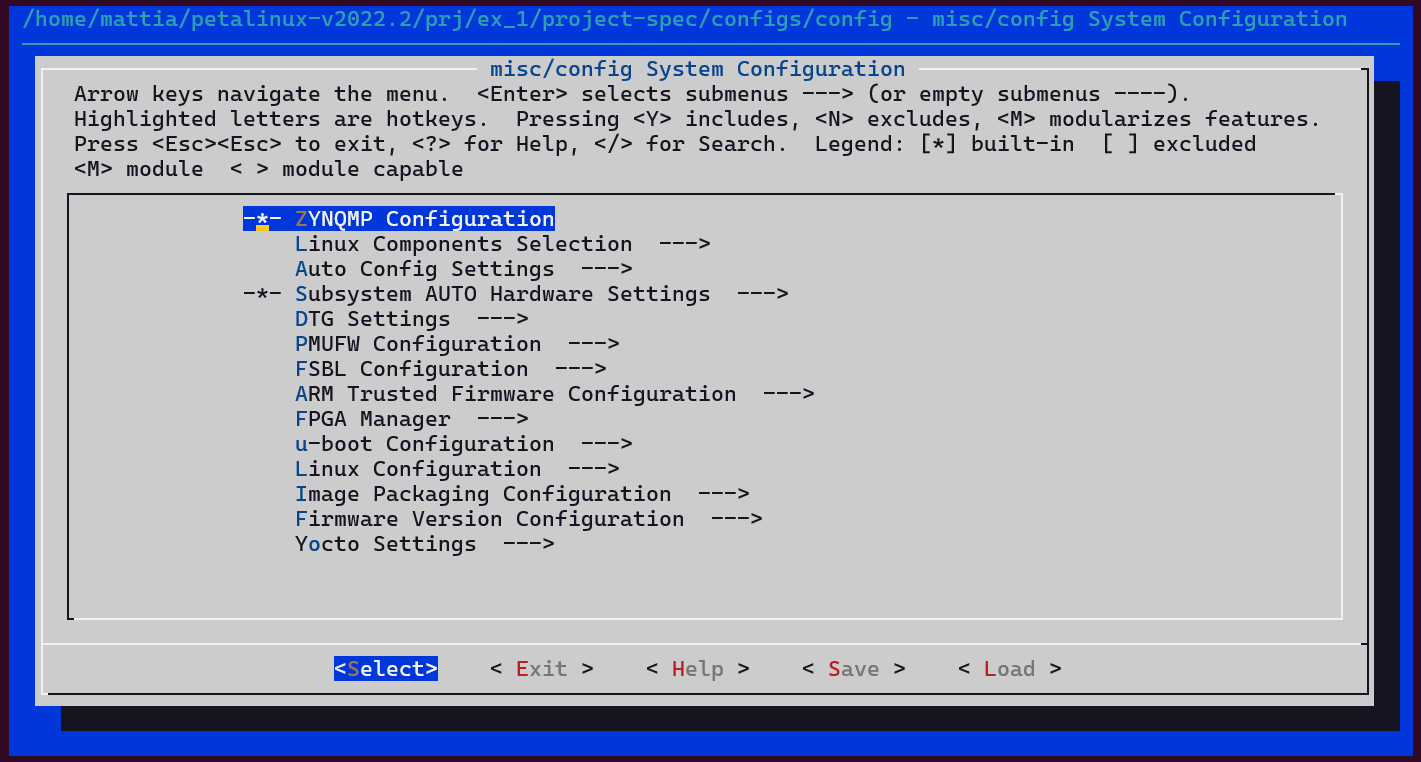
\includegraphics[width=0.8\textwidth]{images/prj2_2}
	\caption{Hardware configuration window.}
	\label{fig:prj2_2}
\end{figure}



\subsection{Packages configuration}
\label{subsec:rootfs-packages}
For the projects described in this guide, the root filesystem does not need the complete XRT/OpenCL acceleration stack. The target system must provide the basic Linux utilities, SSH access, native C/C++ compilation tools and the packages required to deploy custom FPGA applications based on FPGA Manager, device-tree overlays and kernel modules. Keeping the root filesystem minimal reduces both build time and image size.

The installation menu will open with the command
\vspace{0.1cm}
\begin{lstlisting}[language=bash]
	petalinux-config -c rootfs	
\end{lstlisting}
\vspace{0.1cm}
from which the following packages are recommended:
\begin{itemize}

	\item \textbf{Filesystem Packages} $\rightarrow$ \textbf{base} $\rightarrow$ \textbf{util-linux}
	
	\item \textbf{Filesystem Packages} $\rightarrow$ \textbf{console} $\rightarrow$ \textbf{utils} $\rightarrow$ \textbf{git} $\rightarrow$ \textbf{[*]git}
	
	\item \textbf{Filesystem Packages} $\rightarrow$ \textbf{console} $\rightarrow$ \textbf{utiles} $\rightarrow$ \textbf{strace}
	
	\item \textbf{Filesystem Packages} $\rightarrow$ \textbf{console} $\rightarrow$ \textbf{network} $\rightarrow$ \textbf{openssh} $\rightarrow$ \textbf{[*]openssh}, \textbf{[*]openssh-sshd}, \textbf{[*]openssh-sftp-server}
	
	\item \textbf{Filesystem Packages} $\rightarrow$ \textbf{misc} $\rightarrow$ \textbf{packagegroup-core-buildessential} $\rightarrow$ \textbf{[*]packagegroup-core-buildessential}
	
	\item \textbf{Filesystem Packages} $\rightarrow$ \textbf{misc} $\rightarrow$ \textbf{gcc-runtime} $\rightarrow$ \textbf{[*]libstdc++}
	
	\item \textbf{Filesystem Packages} $\rightarrow$ \textbf{misc} $\rightarrow$ \textbf{gdb} $\rightarrow$ \textbf{[*]gdb}
	
	\item \textbf{Filesystem Packages} $\rightarrow$ \textbf{misc} $\rightarrow$ \textbf{glibc} $\rightarrow$ \textbf{[*]glibc}, \textbf{[*]ldd}
	
	\item \textbf{PetaLinux Package Groups} $\rightarrow$ \textbf{packagegroup-petalinux} $\rightarrow$ \textbf{[*]packagegroup-petalinux}
\end{itemize}

This configuration provides the following features:
\begin{itemize}
	\item basic Linux command-line functionality;
	\item SSH remote access to the board;
	\item native C/C++ compilation directly on the KR260;
	\item basic debugging tools such as \texttt{gdb}, \texttt{dmesg} and \texttt{strace};
	\item FPGA Manager support for loading a \texttt{.bin} bitstream at run time;
	\item support for deploying device-tree overlays (\texttt{.dtbo});
	\item support for loading custom kernel modules (\texttt{.ko});
	\item support for the DMA-based user-space applications discussed in Chapter~\ref{ch:dma}.
\end{itemize}

The following packages are not required for the DMA implementation presented in this guide and can be disabled unless OpenCL/XRT acceleration, graphics or multimedia applications are explicitly needed:
\begin{itemize}
	\item \textbf{xrt}, \textbf{xrt-dev};
	\item \textbf{zocl};
	\item \textbf{opencl-headers};
	\item \textbf{opencl-clhpp}, \textbf{opencl-clhpp-dev};
	\item \textbf{libdrm}, \textbf{libdrm-tests}, \textbf{libdrm-kms};
	\item \textbf{bootgen}, \textbf{bootgen-dev};
	\item \textbf{dnf};
	\item \textbf{gcr}, \textbf{gcr-dev};
	\item \textbf{packagegroup-petalinux-gstreamer};
	\item \textbf{packagegroup-petalinux-opencv};
	\item \textbf{packagegroup-petalinux-v4lutils};
	\item \textbf{packagegroup-petalinux-x11}.
\end{itemize}

\begin{figure}[h!t!]
	\centering
	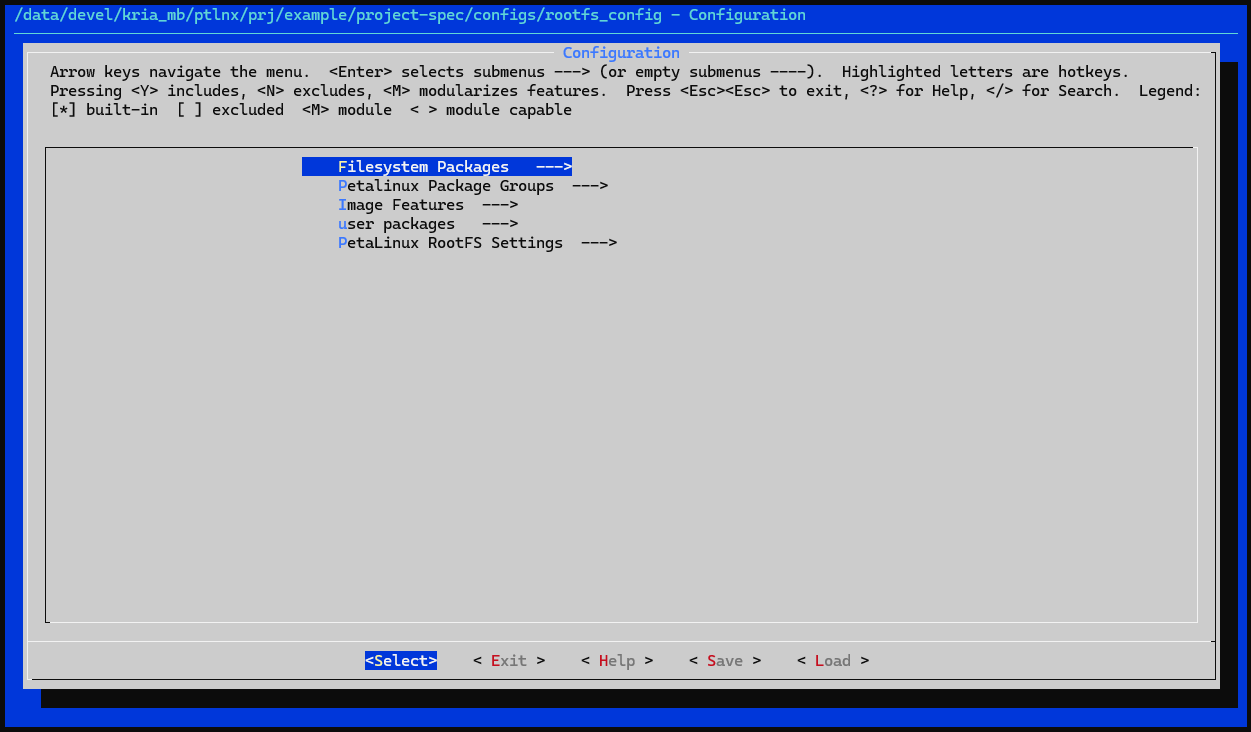
\includegraphics[width=0.8\textwidth]{images/prj2_3}
	\caption{rootfs configuration window.}
	\label{fig:prj2_3}
\end{figure}
After having installed all the needed packages, it is time to rebuild the project with the command
\vspace{0.1cm}
\begin{lstlisting}[language=bash]
	petalinux-build
\end{lstlisting}
\vspace{0.1cm}
In the case of building failure with error messages not related to the implementation, try to clear out the current files by typing
\vspace{0.1cm}
\begin{lstlisting}[language=bash]
	petalinux-config -x mrproper	
\end{lstlisting}
\vspace{0.1cm}
command which is used to deep cleaning the workspace, similar to how it's used in the Linux kernel build system.


\subsection{Board booting}
Since the board boots from a SD card, the system configuration just created has to be converted into a bootable image for the card itself. First step to carry out is the creation of the image files, which are then to be flashed into the SD card. To do so, after the project build, the command is (on the same line)
\vspace{0.1cm}
\begin{lstlisting}[language=bash]
	petalinux-package --boot --fsbl <zynqmp_fsbl.elf> --fpga <path_to_bitstream> --u-boot	
\end{lstlisting}
\vspace{0.1cm}
in which the .elf file is usually located under the path \textit{images/linux/}. The second step is to create a .wic image for the SD card to be flashed in. The command to do that is (on the same line)
\vspace{0.1cm}
\begin{lstlisting}[language=bash]
	petalinux-package --wic --images-dir images/linux/ --bootfiles "ramdisk.cpio.gz.u-boot,boot.scr,Image,system.dtb,system-zynqmp-sck-kr-g-revB.dtb" --disk-name "sda"	
\end{lstlisting}
\vspace{0.1cm}
from which the .wic image will be generated and found in the same folder as the .elf file. To flash the SD card make use of a third-part software, such as balenaEtcher or something similar. Once the flash is done, insert the SD in the board and power it up. With a third part software, such as PuTTY, connect to the serial port (Baud Rate 115200). The system will require to inset some credential. 


\subsection{SSH connection}
Once the board is connected through a serial terminal and the Ethernet cable is plugged in, it is possible to find out the IP address associated to the device by typing
\vspace{0.1cm}
\begin{lstlisting}[language=bash]
	ip a
\end{lstlisting}
\vspace{0.1cm}
Once the IP is known, it is possible to connect to the board via SSH protocol:
\vspace{0.1cm}
\begin{lstlisting}[language=bash]
	ssh board_name@ip_address
\end{lstlisting}
\vspace{0.1cm}


\section{FPGA programming}
So far, the FPGA is not yet programmed. Besides the JTAG procedure, also the On-Run programming is of use: it allows for more flexibility and has the advantage to let the FPGA to be programmed even when the system is running, without the need to repeat all the steps previously explained. To actually program the FPGA after the system is booted, there is the need to the .bin file needs to be "manually" loaded into the FPGA through the FPGA manager. Through SSH copy the .bin file in the /lib/firmware path and to program the FPGA type 
\begin{lstlisting}[language=bash]
	sudo sh -c 'echo "bin_file" > /sys/class/fpga_manager/fpga0/firmware'	\end{lstlisting}
The .bin file can be automatically generated by Vivado when writing the bitstream file. Go to \textbf{Settings}, then \textbf{Bitstream} and check the .bin box.